\documentclass[tikz,border=8pt]{standalone}
% Shared look for every TikZ diagram. Load with \input{../../tools/tikz-style.tex}
\usepackage[T1]{fontenc}
\usepackage{lmodern}
\renewcommand{\sfdefault}{lmr}  % diagrams use the same serif as the text
\usetikzlibrary{arrows.meta, positioning, shapes.geometric, calc, fit, backgrounds}
\definecolor{cblue}{HTML}{4C78A8}
\definecolor{corange}{HTML}{F58518}
\definecolor{cgreen}{HTML}{54A24B}
\definecolor{cred}{HTML}{E45756}
\definecolor{cpurple}{HTML}{B279A2}
\definecolor{cgrey}{HTML}{6B6B6B}
\tikzset{
  every picture/.style={font=\sffamily, line width=1.2pt},
  box/.style={draw=#1, fill=#1!12, rounded corners=4pt, align=center, inner sep=7pt, minimum height=1.1cm},
  box/.default=cgrey,
  arrow/.style={-{Stealth[length=3mm]}, draw=cgrey, line width=1.4pt},
  title/.style={font=\sffamily\bfseries\Large},
  note/.style={font=\sffamily\small, text=cgrey, align=center},
}
\AtBeginDocument{\hyphenpenalty=10000 \exhyphenpenalty=10000}

\begin{document}
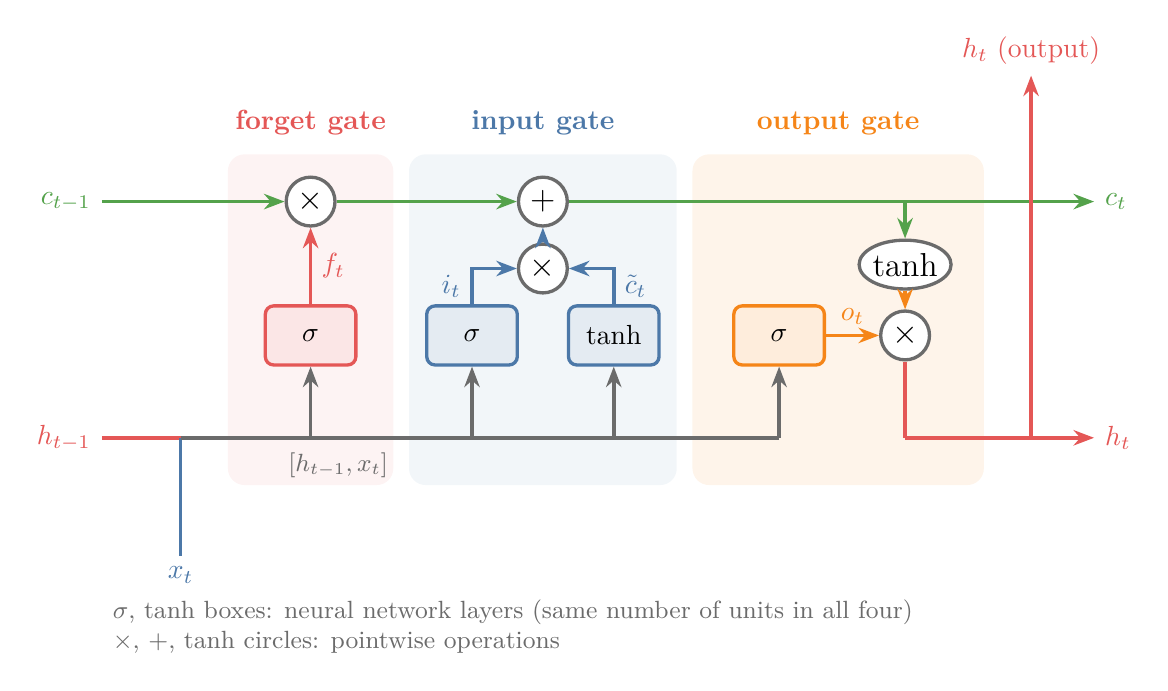
\begin{tikzpicture}[
  layer/.style={draw=#1, fill=#1!15, rounded corners=3pt, minimum width=1.15cm, minimum height=0.75cm, font=\sffamily},
  op/.style={circle, draw=cgrey, fill=white, minimum size=0.62cm, inner sep=0pt, font=\sffamily\large},
  line/.style={-{Stealth[length=2.6mm]}, line width=1.3pt}]
  % gate regions
  \fill[cred!7, rounded corners=6pt] (1.0,-0.6) rectangle (3.1,3.6);
  \fill[cblue!7, rounded corners=6pt] (3.3,-0.6) rectangle (6.7,3.6);
  \fill[corange!9, rounded corners=6pt] (6.9,-0.6) rectangle (10.6,3.6);
  \node[font=\sffamily\bfseries, text=cred] at (2.05,4.0) {forget gate};
  \node[font=\sffamily\bfseries, text=cblue] at (5.0,4.0) {input gate};
  \node[font=\sffamily\bfseries, text=corange] at (8.75,4.0) {output gate};
  % cell-state line
  \node[op] (fx) at (2.05,3) {$\times$};
  \node[op] (plus) at (5.0,3) {$+$};
  \draw[line, draw=cgreen] (-0.6,3) node[left, text=cgreen] {$c_{t-1}$} -- (fx);
  \draw[line, draw=cgreen] (fx) -- (plus);
  \draw[line, draw=cgreen] (plus) -- (12.0,3) node[right, text=cgreen] {$c_t$};
  % input bus: h_{t-1} and x_t joined
  \draw[line width=1.3pt, draw=cred] (-0.6,0) node[left, text=cred] {$h_{t-1}$} -- (0.4,0);
  \draw[line width=1.3pt, draw=cblue] (0.4,-1.5) node[below, text=cblue] {$x_t$} -- (0.4,0);
  \draw[line width=1.3pt, draw=cgrey] (0.4,0) -- (8.0,0);
  \node[note, anchor=north] at (2.4,-0.05) {$[h_{t-1}, x_t]$};
  % four layers
  \node[layer=cred] (f) at (2.05,1.3) {$\sigma$};
  \node[layer=cblue] (i) at (4.1,1.3) {$\sigma$};
  \node[layer=cblue] (ct) at (5.9,1.3) {tanh};
  \node[layer=corange] (o) at (8.0,1.3) {$\sigma$};
  \foreach \n in {f,i,ct,o} \draw[line, draw=cgrey] (\n |- 0,0) -- (\n);
  % forget path
  \draw[line, draw=cred] (f) -- node[right, text=cred] {$f_t$} (fx);
  % input path
  \node[op] (ix) at (5.0,2.15) {$\times$};
  \draw[line, draw=cblue] (i) |- node[pos=0.25, left, text=cblue] {$i_t$} (ix);
  \draw[line, draw=cblue] (ct) |- node[pos=0.25, right, text=cblue] {$\tilde{c}_t$} (ix);
  \draw[line, draw=cblue] (ix) -- (plus);
  % output path
  \node[op, ellipse, minimum width=1.0cm] (th) at (9.6,2.2) {tanh};
  \node[op] (ox) at (9.6,1.3) {$\times$};
  \draw[line, draw=cgreen] (9.6,3) -- (th);
  \draw[line, draw=corange] (th) -- (ox);
  \draw[line, draw=corange] (o) -- node[above, text=corange] {$o_t$} (ox);
  \draw[line width=1.3pt, draw=cred] (ox) -- (9.6,0);
  \draw[line, draw=cred] (9.6,0) -- (12.0,0) node[right, text=cred] {$h_t$};
  \draw[line, draw=cred] (11.2,0) -- (11.2,4.6) node[above, text=cred] {$h_t$ (output)};
  % legend
  \node[note, anchor=west, align=left] at (-0.6,-2.4) {$\sigma$, tanh boxes: neural network layers (same number of units in all four)\\$\times$, $+$, tanh circles: pointwise operations};
\end{tikzpicture}
\end{document}
